% ===================================================================
%  Week 12 — Persian lecture notes — From Features to Machine Learning
% ===================================================================
\documentclass[12pt,a4paper]{article}
% ===================================================================
%  Shared preamble for Persian lecture notes (Image Processing).
%  Compile with XeLaTeX.  Body = Persian (RTL), code/math = LTR.
% ===================================================================

\usepackage{geometry}
\geometry{a4paper,margin=2.4cm}
\usepackage{amsmath,amssymb}
\usepackage{graphicx}
\usepackage{xcolor}
\usepackage{listings}
\usepackage{tcolorbox}
\usepackage{booktabs}
\usepackage{array}
\usepackage{enumitem}
\usepackage{hyperref}
\tcbuselibrary{skins,breakable}

% ---- Persian / RTL --------------------------------------------------
\usepackage{xepersian}
\settextfont{IRNazli}
\setlatintextfont{Latin Modern Roman}
\setdigitfont{IRNazli}
% More generous leading + paragraph spacing (Persian reads better with air).
\linespread{1.5}
\setlength{\parskip}{0.7em}

% ---- Colours --------------------------------------------------------
\definecolor{coursePrimary}{HTML}{1B4965}
\definecolor{courseAccent}{HTML}{E76F51}
\definecolor{courseGood}{HTML}{2A9D8F}
\definecolor{courseBad}{HTML}{C0392B}
\definecolor{courseInfo}{HTML}{2980B9}
\definecolor{codeBg}{HTML}{F5F6FA}
\definecolor{codeKw}{HTML}{8E44AD}
\definecolor{codeStr}{HTML}{2A9D8F}
\definecolor{codeCom}{HTML}{7F8C8D}

\hypersetup{colorlinks=true,linkcolor=courseInfo,urlcolor=courseInfo,citecolor=courseInfo}

% ---- Code listings (Python built in) -------------------------------
\lstdefinestyle{course}{
  backgroundcolor=\color{codeBg},
  basicstyle=\ttfamily\small,
  keywordstyle=\color{codeKw}\bfseries,
  stringstyle=\color{codeStr},
  commentstyle=\color{codeCom}\itshape,
  numberstyle=\tiny\color{codeCom},
  numbers=left, numbersep=7pt,
  showstringspaces=false, breaklines=true,
  tabsize=4, columns=fullflexible, frame=single,
  rulecolor=\color{gray!30}, keepspaces=true, upquote=true, language=Python,
}
\lstset{style=course}
\lstdefinelanguage{bash}{
  keywords={cd,pip,python,venv,source,import}, sensitive=true,
  morecomment=[l]{\#}, morestring=[b]', morestring=[b]",
}
\newenvironment{ltrcode}{\begin{LTR}}{\end{LTR}}

% ---- Callout boxes (Persian titles) --------------------------------
\newtcolorbox{yaddasht}{colback=courseInfo!8,colframe=courseInfo,
  title={\textbf{یادداشت}},boxrule=0.6pt,right=6pt,left=6pt,breakable}
\newtcolorbox{nokte}{colback=courseAccent!10,colframe=courseAccent,
  title={\textbf{نکتهٔ کلیدی}},boxrule=0.6pt,right=6pt,left=6pt,breakable}
\newtcolorbox{hoshdar}{colback=courseBad!8,colframe=courseBad,
  title={\textbf{هشدار / دام}},boxrule=0.6pt,right=6pt,left=6pt,breakable}
\newtcolorbox{riyazi}{colback=coursePrimary!6,colframe=coursePrimary,
  title={\textbf{ریاضیات}},boxrule=0.6pt,right=6pt,left=6pt,breakable}
\newtcolorbox{tamrin}{colback=courseGood!8,colframe=courseGood,
  title={\textbf{تمرین}},boxrule=0.6pt,right=6pt,left=6pt,breakable}

% ---- Header helper --------------------------------------------------
\newcommand{\coursemeta}[2]{%
  \begin{center}
  {\large\textbf{پردازش تصویرِ کاربردی}}\\[2pt]
  {\color{coursePrimary}\rule{\linewidth}{1pt}}\\[4pt]
  {\Large\textbf{#1}}\\[3pt]
  {\small جزوهٔ درس — #2}
  \end{center}\vspace{4pt}
}


\begin{document}
\coursemeta{جلسهٔ ۱۲ — از ویژگی تا یادگیریِ ماشین (Features $\rightarrow$ Machine Learning)}{هفتهٔ دوازدهم}

\section*{نگاهِ کلی به این جلسه}

این جلسه یک نقطهٔ عطف در درس است. تا هفتهٔ ۱۱، \emph{ما} هر گام را طراحی می‌کردیم: کدام فیلتر، کدام آستانه، کدام لبه، کدام تبدیل. از این هفته رویکرد عوض می‌شود: به‌جای طراحیِ دستیِ قاعده، به کامپیوتر \emph{مثال‌های برچسب‌دار} می‌دهیم و می‌گذاریم خودش قاعدهٔ تصمیم را «یاد بگیرد». این همان \textbf{یادگیریِ ماشین} (Machine Learning) است. پلی که پردازش تصویرِ کلاسیک را به یادگیریِ ماشین وصل می‌کند، همان مفهومِ آشنای «ویژگی» است: تصویر را به یک بردارِ ویژگی تبدیل می‌کنیم و سپس یک \textbf{طبقه‌بند} (classifier) روی این بردارها آموزش می‌دهیم.

\begin{yaddasht}
تسکِ واقعیِ امروز: طبقه‌بندیِ مدلِ خودروهای ایرانی (پژو ۲۰۶ در برابرِ ۴۰۵ در برابرِ دنا) از روی ویژگی‌های \textbf{HOG}، با استفاده از تصاویرِ واقعیِ شما در \texttt{E:/data/Vehicle\_classes}. این یک مسئلهٔ سختِ واقعی است و — همان‌طور که خواهیم دید — نتیجه‌اش درسِ صادقانه‌ای دربارهٔ محدودیت‌های ویژگیِ دست‌طراحی به ما می‌دهد.
\end{yaddasht}

\subsection*{یک تشبیهِ ساده}

فرض کنید می‌خواهید به کودکی یاد بدهید سیب را از پرتقال تشخیص دهد. دو راه دارید. راهِ اول (کلاسیک): به او \emph{قاعده} بدهید — «اگر گِرد و قرمز است سیب، اگر گِرد و نارنجی با پوستِ ناهموار است پرتقال». راهِ دوم (یادگیری): ده‌ها سیب و پرتقالِ برچسب‌دار نشانش دهید و بگذارید خودش قاعده را کشف کند. یادگیریِ ماشین راهِ دوم است. اما یک نکتهٔ ظریف: در راهِ دوم هم باید تصمیم بگیرید کودک به \emph{چه چیزی} نگاه کند — رنگ؟ شکل؟ بافت؟ این «چه چیزی» همان ویژگی است. امروز ویژگی را ما انتخاب می‌کنیم (HOG) و فقط قاعده را واگذار می‌کنیم؛ در یادگیریِ عمیق، انتخابِ ویژگی هم به ماشین واگذار می‌شود.

\section{خط‌لولهٔ کلاسیکِ شناسایی}

تقریباً همهٔ سامانه‌های شناساییِ تصویر تا حدودِ سالِ ۲۰۱۲ این ساختار را داشتند:

\begin{enumerate}
  \item \textbf{تصویرِ ورودی} $\rightarrow$
  \item \textbf{استخراجِ ویژگی} (تبدیلِ پیکسل‌ها به یک بردارِ فشرده) $\rightarrow$
  \item \textbf{طبقه‌بند} (تابعی آموخته‌شده که بردار را به برچسب می‌نگارد) $\rightarrow$
  \item \textbf{پیش‌بینی} (۲۰۶ / ۴۰۵ / دنا).
\end{enumerate}

\begin{nokte}
نکتهٔ تاریخیِ مهم: در این خط‌لوله، \emph{ویژگی‌ها دست‌طراحی} بودند (توسطِ انسان) و فقط \emph{طبقه‌بند} یاد گرفته می‌شد. در هفته‌های ۱۳ و ۱۴ خواهیم دید که یادگیریِ عمیق این را تغییر داد: خودِ ویژگی‌ها هم از داده یاد گرفته می‌شوند.
\end{nokte}

\subsection{چرا پیکسل‌های خام را مستقیم نمی‌دهیم؟}

یک تصویرِ $۹۶\times۹۶$ برابرِ ۹۲۱۶ عدد است — بسیار بزرگ. مهم‌تر: پیکسل‌های خام \textbf{ناوردا} نیستند. اگر همان خودرو را ۵ پیکسل جابه‌جا کنیم یا نور کمی عوض شود، تقریباً همهٔ ۹۲۱۶ عدد تغییر می‌کنند، در حالی که خودرو همان خودروست. یک طبقه‌بند که مستقیم روی پیکسل‌ها کار کند، این جابه‌جاییِ بی‌اهمیت را «تفاوت» می‌بیند.

\begin{yaddasht}
ویژگی‌های خوب (HOG، هیستوگرامِ رنگ، ORB) تصویر را به برداری فشرده، پایدار و معنادار تبدیل می‌کنند. هدفِ نهایی این است که کلاس‌ها در «فضای ویژگی» \textbf{جداپذیر} (separable) شوند: چیزهای شبیه به هم نزدیکِ هم بیفتند و چیزهای متفاوت دور از هم.
\end{yaddasht}

\subsection{HOG: هیستوگرامِ گرادیان‌های جهت‌دار}

\textbf{HOG} (Histogram of Oriented Gradients) یکی از موفق‌ترین ویژگی‌های دست‌طراحی است. ایده ساده است: تصویر را به سلول‌های کوچک تقسیم کن و در هر سلول، \emph{جهتِ} گرادیان‌ها را در یک هیستوگرام بشمار. نتیجه یک «امضای شکلیِ» فشرده است.

\begin{center}
  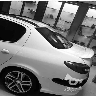
\includegraphics[width=0.4\linewidth]{../assets/sample_gray.png}\hfill
  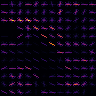
\includegraphics[width=0.4\linewidth]{../assets/hog_vis.png}\\
  {\small چپ: یک پژو ۲۰۶ واقعی \quad راست: نقشهٔ HOGِ آن (جهتِ لبه‌ها در هر سلول)}
\end{center}

\begin{riyazi}
چرا HOG برای شکل خوب کار می‌کند؟ خودروها در \emph{شکل} تفاوت دارند (خطِ سقف، چراغ‌ها، جلوپنجره) و این تفاوت‌ها در جهتِ گرادیان‌ها ثبت می‌شوند. هیستوگرام‌کردن در هر سلول، تحمل نسبت به جابه‌جاییِ کوچک و تغییرِ نور می‌دهد. ترکیبِ HOG + SVMِ خطی سال‌ها بهترین روش برای تشخیصِ عابر و خودرو بود.
\end{riyazi}

HOG مقدارِ دقیقِ پیکسل‌ها را دور می‌ریزد و فقط نگه می‌دارد که «لبه‌ها به کدام سو اشاره می‌کنند» — و همین جوهرهٔ شکل است.

\subsection{HOG گام‌به‌گام (شهودِ عددی)}

بیایید دقیق‌تر ببینیم HOG چه می‌کند:

\begin{enumerate}
  \item گرادیانِ افقی $G_x$ و عمودی $G_y$ هر پیکسل را حساب کن (مثلِ سوبلِ هفتهٔ ۵).
  \item بزرگی $m=\sqrt{G_x^2+G_y^2}$ و جهت $\theta=\arctan(G_y/G_x)$ را به دست آور.
  \item تصویر را به سلول‌های مثلاً $۸\times۸$ تقسیم کن. در هر سلول، جهت‌ها را به ۹ سطلِ ($۰$ تا $۱۸۰$ درجه) تقسیم و با وزنِ بزرگی جمع کن — این یک هیستوگرامِ ۹‌تایی می‌دهد.
  \item بلوک‌هایی از $۲\times۲$ سلول را کنارِ هم نرمال کن (تا نسبت به تغییرِ نور مقاوم شود).
\end{enumerate}

\begin{riyazi}
مثالِ عددیِ کوچک: اگر در یک سلول بیشترِ لبه‌ها عمودی باشند (مثلِ ستونِ درِ خودرو)، سطلِ نزدیک به $۹۰^\circ$ مقدارِ بزرگی می‌گیرد و بقیهٔ سطل‌ها کوچک می‌مانند. پس همان سلول با برداری مثلِ $[۰٫۱, ۰٫۱, \dots, ۰٫۸, \dots]$ توصیف می‌شود که «اینجا لبهٔ عمودیِ قوی هست» را کد می‌کند. کلِ تصویر می‌شود به‌هم‌چسباندنِ این هیستوگرام‌های سلولی.
\end{riyazi}

\begin{yaddasht}
به همین دلیل HOG «امضای شکل» است: می‌گوید در هر ناحیه لبه‌ها به کدام سو می‌روند، بی‌آنکه به روشناییِ مطلق حساس باشد. برای تصویرِ $۹۶\times۹۶$ ما، این کار برداری با حدودِ ۹۰۰ عدد تولید کرد.
\end{yaddasht}

\section{طبقه‌بند چه چیزی یاد می‌گیرد؟}

با داشتنِ بردارهای ویژگیِ برچسب‌دار، طبقه‌بند یک \textbf{مرزِ تصمیم} (decision boundary) بینِ کلاس‌ها یاد می‌گیرد. دو طبقه‌بندِ ساده که امروز استفاده می‌کنیم:

\begin{itemize}
  \item \textbf{k نزدیک‌ترین همسایه (k-NN):} برای برچسب‌زدنِ یک نقطه، به $k$ نقطهٔ نزدیکش در دادهٔ آموزش نگاه کن و رأیِ اکثریت را بگیر. عملاً داده را «حفظ» می‌کند.
  \item \textbf{ماشینِ بردارِ پشتیبان (SVM):} مرزی پیدا می‌کند که بیشترین \textbf{حاشیه} (margin) را بینِ کلاس‌ها داشته باشد. با کرنلِ RBF می‌تواند مرزهای منحنی هم بسازد.
\end{itemize}

\begin{nokte}
هر دو طبقه‌بند به فضای ویژگیِ جداپذیر نیاز دارند. اگر ویژگی‌ها کلاس‌ها را از هم جدا نکنند، هیچ طبقه‌بندی نمی‌تواند معجزه کند — «آشغال ورودی، آشغال خروجی».
\end{nokte}

\subsection{k-NN با یک مثالِ عددی}

بیایید k-NN را روی یک مثالِ اسباب‌بازی ببینیم. فرض کنید ویژگی‌ها دوبُعدی‌اند و ۴ نمونهٔ آموزش داریم:

\begin{riyazi}
$A(1,1)\!\to$ کلاسِ ۰,\quad $B(1,2)\!\to$ کلاسِ ۰,\quad $C(5,5)\!\to$ کلاسِ ۱,\quad $D(6,5)\!\to$ کلاسِ ۱.\\[3pt]
نقطهٔ جدید $P(2,2)$ را طبقه‌بندی کنیم با $k=۳$. فاصله‌ها:
\[
d(P,A)=\sqrt{1{+}1}=1.41,\ d(P,B)=1,\ d(P,C)=\sqrt{9{+}9}=4.24,\ d(P,D)=5
\]
سه همسایهٔ نزدیک: $B, A, C$ با کلاس‌های $۰, ۰, ۱$. رأیِ اکثریت $\to$ کلاسِ ۰.
\end{riyazi}

\begin{nokte}
می‌بینید که k-NN هیچ «آموزشی» به‌معنای واقعی ندارد؛ فقط داده را ذخیره می‌کند و در زمانِ پیش‌بینی فاصله‌ها را حساب می‌کند. به همین دلیل آموزشش فوری اما پیش‌بینی‌اش کند است (باید با همهٔ نقاط مقایسه کند). انتخابِ $k$ هم مهم است: $k$ خیلی کوچک به نویز حساس، $k$ خیلی بزرگ مرزها را بیش‌از‌حد صاف می‌کند.
\end{nokte}

\subsection{کلاس‌های ما در فضای ویژگی}

برای دیدنِ اینکه آیا کلاس‌ها اصلاً جداپذیرند، بردارهای ۹۰۰‌بُعدیِ HOG را با PCA به ۲ بُعد فشرده و رسم کردیم:

\begin{center}
  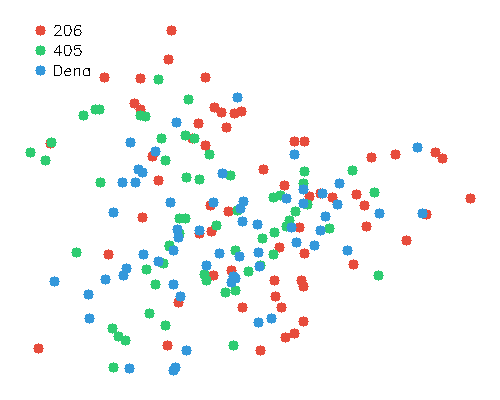
\includegraphics[width=0.44\linewidth]{../assets/feature_space.png}\\
  {\small هر نقطه یک خودروی واقعی است؛ سه رنگ = سه مدل. کلاس‌ها زیاد هم‌پوشانی دارند}
\end{center}

می‌بینید که کلاس‌ها به‌شدت درهم‌اند. این سه مدلِ خودرو واقعاً شبیهِ هم‌اند (هر سه سدانِ متوسطِ ایرانی)، پس این یک مسئلهٔ \emph{سخت} است. این نمودار پیش‌بینی می‌کند که دقتِ بالا دشوار خواهد بود — و همین‌طور هم شد.

\subsection{ویژگی‌های کلاسیکِ دیگر}

HOG تنها ویژگیِ ممکن نیست. بسته به مسئله، ویژگی‌های دیگری هم داریم:

\begin{itemize}
  \item \textbf{هیستوگرامِ رنگ:} توزیعِ رنگ‌ها را می‌شمارد. برای تفکیکِ اشیایی که رنگِ متفاوت دارند عالی است (مثلاً میوهٔ قرمز در برابرِ سبز)، اما به شکل بی‌اعتناست.
  \item \textbf{LBP (الگوی باینریِ محلی):} بافت را کد می‌کند؛ برای تشخیصِ بافتِ سطح (پارچه، دیوار، پوست) مفید است.
  \item \textbf{کیسهٔ کلماتِ بصری (Bag of Visual Words):} توصیف‌گرهای ORB/SIFT را (از هفتهٔ ۱۰) خوشه‌بندی می‌کند و هر تصویر را با هیستوگرامِ «کلمات بصری» توصیف می‌کند — پلی زیبا بینِ هفتهٔ ۱۰ و طبقه‌بندی.
\end{itemize}

\begin{nokte}
اغلب بهترین نتیجه از \emph{ترکیبِ} چند ویژگی به دست می‌آید: مثلاً HOG (شکل) + هیستوگرامِ رنگ. این را «الحاقِ ویژگی» (feature concatenation) می‌گویند: دو بردار را به هم می‌چسبانیم و طبقه‌بند از هر دو استفاده می‌کند.
\end{nokte}

\section{تقسیمِ آموزش/آزمون: قاعدهٔ طلایی}

مهم‌ترین اصلِ روش‌شناسیِ یادگیریِ ماشین: داده را به دو بخش تقسیم کن. روی بخشِ \textbf{آموزش} (train) طبقه‌بند را یاد بده، و روی بخشِ \textbf{آزمونِ} (test) دیده‌نشده ارزیابی کن.

\begin{hoshdar}
هرگز دقت را روی داده‌ای که مدل دیده گزارش نکنید. مدل می‌تواند داده را حفظ کند و روی آن ۱۰۰٪ بگیرد، بی‌آنکه چیزی «یاد گرفته» باشد. آن عدد برای استفادهٔ واقعی بی‌معنی است.
\end{hoshdar}

ما ۷۰٪ آموزش و ۳۰٪ آزمون گرفتیم، به‌صورتِ \textbf{طبقه‌بندی‌شده} (stratified) — یعنی نسبتِ هر کلاس در هر دو بخش یکسان نگه داشته شد تا ارزیابی منصفانه باشد.

\section{نتایجِ واقعی و یک درسِ صادقانه}

نتایجِ واقعیِ اجرا روی داده‌های شما:

\begin{center}
\begin{tabular}{@{}lcc@{}}
\hline
\textbf{طبقه‌بند} & \textbf{دقتِ آموزش} & \textbf{دقتِ آزمون} \\
\hline
k-NN ($k{=}۵$) & ۰٫۶۵ & ۰٫۴۳ \\
SVM (کرنلِ RBF) & ۱٫۰۰ & ۰٫۴۸ \\
\hline
\end{tabular}
\end{center}

شانسِ تصادفی برای ۳ کلاس $۰٫۳۳$ است، پس هر دو طبقه‌بند بهتر از شانس‌اند. اما به SVM دقت کنید: \textbf{۱۰۰٪ روی آموزش، ۴۸٪ روی آزمون}. این شکافِ بزرگ یک نام دارد: \textbf{بیش‌برازش} (overfitting).

\subsection{بیش‌برازش چیست؟}

بیش‌برازش یعنی مدل به‌جای یادگرفتنِ الگوی واقعی، ویژگی‌های تصادفی و نویزِ دادهٔ آموزش را حفظ کرده است.

\begin{itemize}
  \item \textbf{نشانه:} دقتِ آموزش خیلی بیشتر از دقتِ آزمون (اینجا ۱٫۰۰ در برابرِ ۰٫۴۸).
  \item \textbf{درمان‌ها:} دادهٔ بیشتر، مدلِ ساده‌تر، منظم‌سازی (regularization)، یا ویژگی‌های بهتر و ناوردا‌تر.
\end{itemize}

\begin{riyazi}
چرا SVMِ ما این‌قدر بد بیش‌برازش کرد؟ فقط ۱۲۶ بردارِ آموزش داشتیم، هر کدام ۹۰۰‌بُعدی — یعنی ابعادِ ویژگی بسیار بیشتر از تعدادِ نمونه‌هاست. یک SVMِ RBF با $C$ بزرگ می‌تواند مرز را آن‌قدر خم کند که هر نقطهٔ آموزش را دقیق در بر بگیرد. نتیجه: ۱٫۰۰ روی آموزش، اما مرزی که به نویز کوک شده و روی آزمون فرو می‌ریزد. «ابعادِ بیشتر از نمونه‌ها» یک پرچمِ قرمز است.
\end{riyazi}

\begin{nokte}
درمان‌های عملی برای همین مورد: کاهشِ $C$ (منظم‌سازیِ بیشتر)، کاهشِ ابعاد با PCA پیش از طبقه‌بندی، یا جمع‌آوریِ دادهٔ آموزشِ بیشتر. مدلی که روی آموزش کامل و روی آزمون متوسط است، چیزِ اشتباهی یاد گرفته.
\end{nokte}

\section{ماتریسِ درهم‌ریختگی}

یک عددِ دقت کافی نیست؛ باید بدانیم \emph{کدام} کلاس‌ها اشتباه می‌شوند. \textbf{ماتریسِ درهم‌ریختگی} (confusion matrix) این را نشان می‌دهد:

\begin{center}
  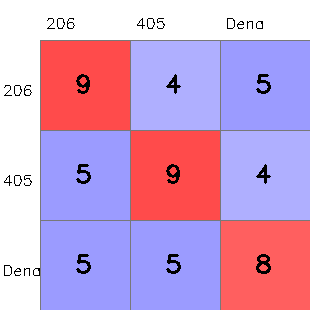
\includegraphics[width=0.36\linewidth]{../assets/confusion.png}\\
  {\small سطر = کلاسِ واقعی، ستون = پیش‌بینی؛ قطر = درست، خارجِ قطر = خطاها}
\end{center}

خانه‌های قطرِ اصلی نمونه‌های درست‌اند و خانه‌های خارجِ قطر خطاها. این ماتریس می‌گوید مثلاً چند تا ۲۰۶ اشتباهاً ۴۰۵ پیش‌بینی شده‌اند — اطلاعاتی بسیار مفیدتر از یک عددِ دقتِ کلی.

\subsection{سنجه‌های فراتر از دقت}

دقت (accuracy) می‌تواند گمراه‌کننده باشد، به‌خصوص وقتی کلاس‌ها نامتوازن‌اند.

\begin{riyazi}
فرض کنید ۹۶٪ داده «سالم» و ۴٪ «معیوب» است. یک مدل که همیشه «سالم» بگوید ۹۶٪ دقت دارد اما \emph{هیچ} عیبی را نمی‌گیرد — بی‌فایده! سنجه‌های بهتر:
\[
\text{Precision} = \frac{TP}{TP+FP},\quad
\text{Recall} = \frac{TP}{TP+FN},\quad
\text{F1} = \frac{2\,PR}{P+R}
\]
\textbf{صحت} (precision): از موارِد پیش‌بینی‌شده به‌عنوانِ مثبت، چند‌تا درست بود؟ \textbf{فراخوانی} (recall): از موارِد واقعاً مثبت، چند‌تا را گرفتیم؟ \textbf{F1} میانگینِ هارمونیکِ این دو است.
\end{riyazi}

\begin{yaddasht}
همیشه این سنجه‌ها را \emph{به‌ازای هر کلاس} گزارش کنید، نه یک عددِ کلی. در سامانهٔ کنتورِ شما، «نگرفتنِ یک رقمِ اشتباه» (recall پایین) ممکن است بسیار پرهزینه‌تر از یک هشدارِ اضافی باشد.
\end{yaddasht}

\section{مصالحهٔ اریبی-واریانس}

بیش‌برازش بخشی از یک تصویرِ بزرگ‌تر است به نامِ \textbf{مصالحهٔ اریبی-واریانس} (bias-variance tradeoff):

\begin{itemize}
  \item \textbf{اریبیِ بالا (underfitting):} مدل بیش‌از‌حد ساده است و حتی الگوی آموزش را هم نمی‌گیرد. نشانه: هم دقتِ آموزش و هم آزمون پایین.
  \item \textbf{واریانسِ بالا (overfitting):} مدل بیش‌از‌حد پیچیده است و نویز را حفظ می‌کند. نشانه: دقتِ آموزش بالا، آزمون پایین (دقیقاً موردِ SVMِ ما).
  \item \textbf{نقطهٔ مطلوب:} پیچیدگیِ متعادل که هم الگو را می‌گیرد و هم تعمیم می‌یابد.
\end{itemize}

\begin{riyazi}
با افزایشِ پیچیدگیِ مدل، خطای آموزش پیوسته کاهش می‌یابد، اما خطای آزمون ابتدا کم و سپس دوباره زیاد می‌شود (منحنیِ U). هدفِ ما پیدا‌کردنِ کفِ آن U است — نه ساده‌ترین و نه پیچیده‌ترین مدل. ابزارهایی مثلِ اعتبارسنجیِ متقابل به یافتنِ این نقطه کمک می‌کنند.
\end{riyazi}

\begin{yaddasht}
برای مسئلهٔ ما: SVM با $C=۱۰$ در سمتِ واریانسِ بالا بود. کاهشِ $C$ یا کاهشِ ابعادِ ویژگی، مدل را به سمتِ کفِ U می‌بَرَد. این‌ها آزمایش‌هایی هستند که در پروژهٔ این هفته انجام می‌دهید.
\end{yaddasht}

\section{اعتبارسنجیِ متقابل: خودت را گول نزن}

یک تقسیمِ واحدِ آموزش/آزمون نویزی است؛ ممکن است تصادفاً خوش‌شانس یا بدشانس باشید. \textbf{اعتبارسنجیِ متقابلِ k-تایی} (k-fold cross-validation) داده را به $k$ بخش تقسیم می‌کند، $k$ بار آموزش/آزمون می‌گیرد (هر بار یک بخشِ متفاوت به‌عنوانِ آزمون) و میانگین می‌گیرد — برآوردی پایدارتر.

\begin{hoshdar}
پارامترها را روی مجموعهٔ \textbf{اعتبارسنجی} (validation) یا با CV تنظیم کنید، هرگز روی مجموعهٔ آزمون. مجموعهٔ آزمون فقط \emph{یک بار}، در انتهای کار، استفاده می‌شود. اگر بارها به آن نگاه کنید و پارامتر تنظیم کنید، عملاً آن را هم به بخشی از آموزش تبدیل کرده‌اید و دقتِ گزارش‌شده متورم می‌شود.
\end{hoshdar}

\section{نرمال‌سازیِ ویژگی: گامی که فراموش می‌شود}

یک نکتهٔ عملیِ مهم: بسیاری از طبقه‌بندها (به‌ویژه k-NN و SVM) به \emph{مقیاسِ} ویژگی‌ها حساس‌اند. اگر یک ویژگی در بازهٔ ۰ تا ۱۰۰۰ و دیگری در بازهٔ ۰ تا ۱ باشد، فاصلهٔ اقلیدسی عملاً فقط ویژگیِ اول را می‌بیند.

\begin{riyazi}
راه‌حل، \textbf{استانداردسازی} است: هر ویژگی را طوری تبدیل کنیم که میانگینِ صفر و انحرافِ‌معیارِ یک داشته باشد:
\[
x'_j = \frac{x_j - \mu_j}{\sigma_j}
\]
که $\mu_j$ و $\sigma_j$ میانگین و انحرافِ‌معیارِ ویژگیِ $j$ روی دادهٔ \emph{آموزش}‌اند. نکتهٔ حیاتی: این $\mu$ و $\sigma$ را فقط از آموزش حساب کنید و همان‌ها را روی آزمون اعمال کنید — وگرنه اطلاعاتِ آزمون به آموزش نشت می‌کند.
\end{riyazi}

\begin{hoshdar}
یک اشتباهِ بسیار رایج: محاسبهٔ میانگین/انحرافِ‌معیار روی \emph{کلِ} داده پیش از تقسیم. این «نشتِ داده» (data leakage) است و دقتِ گزارش‌شده را به‌طورِ کاذب بالا می‌برد. همیشه اول تقسیم کنید، بعد نرمال‌سازی را روی آموزش برازش دهید.
\end{hoshdar}

خبرِ خوب برای مورد ما: HOG به‌طورِ درونی بلوک‌هایش را نرمال می‌کند، پس مقیاسِ ویژگی‌ها از قبل نسبتاً یکنواخت است. اما برای ویژگی‌های ترکیبی (HOG + رنگ) استانداردسازی ضروری می‌شود.

\section{ژرف‌نگری: مهندسیِ ویژگی در برابرِ یادگیریِ ویژگی}

امروز ما ویژگی‌ها را \emph{مهندسی} کردیم (HOG) و فقط طبقه‌بند را یاد دادیم. سقفِ ۴۸٪ روی خودروهای شبیه‌به‌هم، محدودیتِ ویژگیِ دست‌طراحی را نشان می‌دهد: HOG شکلِ کلی را می‌گیرد اما تفاوت‌های ظریفِ بینِ ۲۰۶ و ۴۰۵ را خوب کد نمی‌کند.

\begin{nokte}
\textbf{یادگیریِ عمیق} (هفته‌های ۱۳ و ۱۴) این را تغییر می‌دهد: خودِ ویژگی‌ها را مستقیماً از پیکسل‌ها یاد می‌گیرد. به‌جای اینکه ما تصمیم بگیریم «جهتِ گرادیان مهم است»، شبکه خودش کشف می‌کند کدام الگوها برای تفکیکِ کلاس‌ها مفیدند. همین، جهشِ دقت در مسائلِ سخت را ممکن می‌کند. پس این جلسه هم یک ابزارِ عملی به شما داد و هم \emph{انگیزهٔ} هفته‌های بعد را روشن کرد.
\end{nokte}

\subsection{چطور ۴۸٪ را بهبود دهیم؟ (یک نقشهٔ آزمایش)}

سقفِ ۴۸٪ پایانِ راه نیست؛ چند آزمایشِ مشخص که در پروژه امتحان می‌کنید:

\begin{itemize}
  \item \textbf{دادهٔ بیشتر:} از ۶۰ به ۳۰۰ تصویر در هر کلاس. معمولاً بیشترین تأثیر را دارد و شکافِ بیش‌برازش را کم می‌کند.
  \item \textbf{کاهشِ $C$:} از ۱۰ به ۱ یا ۰٫۱. مرزِ SVM را ساده‌تر می‌کند؛ دقتِ آموزش پایین می‌آید اما آزمون معمولاً بالا می‌رود.
  \item \textbf{PCA پیش از طبقه‌بندی:} ۹۰۰ بُعد را به مثلاً ۵۰ بُعد کاهش دهید؛ نویز کم و بیش‌برازش مهار می‌شود.
  \item \textbf{ویژگیِ ترکیبی:} HOG + هیستوگرامِ رنگ. اگر مدل‌ها رنگِ رایجِ متفاوت داشته باشند، کمک می‌کند.
  \item \textbf{اعتبارسنجیِ متقابل:} به‌جای یک تقسیم، ۵-تایی؛ برآوردِ دقت پایدارتر و قابلِ اعتمادتر می‌شود.
\end{itemize}

\begin{nokte}
روشِ مهندسی: هر بار \emph{یک} چیز را تغییر دهید و اثرش را روی دقتِ آزمون بسنجید. تغییرِ هم‌زمانِ چند چیز، فهمِ اینکه چه چیزی کمک کرد را غیرممکن می‌کند. این «آزمایشِ کنترل‌شده» هستهٔ کارِ تجربی در یادگیریِ ماشین است.
\end{nokte}

\subsection{پیوند با DocScan}

DocScan باید ارقام را بخواند. یک رقم یک تصویرِ کوچک است و یک طبقه‌بند آن را به یکی از ۰ تا ۹ می‌نگارد. دقیقاً همین خط‌لولهٔ «ویژگی $\rightarrow$ طبقه‌بند» بود که OCRِ کلاسیک با آن کار می‌کرد. هفتهٔ آینده ویژگی‌های دستی را با یک \textbf{CNN} که خودش ویژگی‌ها را یاد می‌گیرد جایگزین می‌کنیم و خواهیم دید دقت چطور جهش می‌کند.

\section{کدِ کاملِ خط‌لوله}

\begin{ltrcode}
\begin{lstlisting}[language=Python]
from sklearn.svm import SVC
from sklearn.model_selection import train_test_split
from sklearn.metrics import accuracy_score, confusion_matrix

X = [hog(gray(img)) for img in images]     # 1) features
Xtr, Xte, ytr, yte = train_test_split(     # 2) split
        X, y, test_size=0.3, stratify=y, random_state=0)
clf = SVC(kernel='rbf', C=10).fit(Xtr, ytr)  # 3) learn
pred = clf.predict(Xte)                       # 4) evaluate
print(accuracy_score(yte, pred))              # HONEST score
print(confusion_matrix(yte, pred))
\end{lstlisting}
\end{ltrcode}

ترتیب همیشه ثابت است: استخراجِ ویژگی $\rightarrow$ تقسیم $\rightarrow$ برازش $\rightarrow$ ارزیابی روی دادهٔ دیده‌نشده.

\section{تمرینِ کلاسی و پاسخ}

\begin{tamrin}
۱) SVMِ ما آموزش ۱٫۰۰ و آزمون ۰٫۴۸ گرفت. نامِ مشکل و دو راهِ کاهشش چیست؟\\
۲) یک آشکارسازِ عیب ۹۶٪ دقت گزارش می‌کند اما عیب‌ها ۴٪ داده‌اند. چرا ممکن است بی‌فایده باشد؟\\
۳) می‌خواهید ۲۰۶ را از ۴۰۵ تفکیک کنید. چه ویژگی‌ای غیر از HOG می‌تواند کمک کند؟
\end{tamrin}

\textbf{پاسخ‌ها:} (۱) \textbf{بیش‌برازش}؛ دادهٔ بیشتر جمع کنید، یا SVM را ساده‌تر/منظم‌تر کنید (کاهشِ $C$)، یا ابعاد را با PCA کم کنید. (۲) پیش‌بینیِ همیشه‌«سالم» ۹۶٪ می‌گیرد اما \textbf{فراخوانیِ صفر} روی عیب‌ها دارد — دقت سنجهٔ اشتباهی است؛ باید precision/recall گزارش شود. (۳) \textbf{هیستوگرامِ رنگ} (مدل‌ها رنگِ رایجِ متفاوت دارند)، اندازه/نسبتِ ابعاد، یا ویژگی‌های ناحیهٔ آرم.

\section{زمینهٔ تاریخی}

یادگیریِ ماشین در بینایی یک‌شبه نیامد. در دهه‌های ۱۹۹۰ و ۲۰۰۰، ترکیب‌هایی مثلِ HOG+SVM یا Haar+AdaBoost (آشکارسازِ چهرهٔ Viola-Jones در ۲۰۰۱) استانداردِ صنعت بودند و در دوربین‌ها و خودروها به کار می‌رفتند. نقطهٔ عطف در سالِ ۲۰۱۲ رخ داد: شبکهٔ AlexNet در مسابقهٔ ImageNet با اختلافِ زیادی همهٔ روش‌های مبتنی‌بر‌ویژگیِ دستی را شکست داد و نشان داد که \emph{یادگرفتنِ ویژگی‌ها} از پیکسل‌ها بسیار قدرتمندتر است. از آن پس، تقریباً همهٔ سامانه‌های شناساییِ پیشرفته به یادگیریِ عمیق کوچ کردند.

\begin{yaddasht}
اما — و این مهم است — روش‌های کلاسیکِ این جلسه هنوز جای خود را دارند: وقتی داده کم است، وقتی به سرعتِ بالا و منابعِ محدود نیاز دارید، یا وقتی قابلیتِ تفسیر مهم است. یک مهندسِ خوب هر دو ابزار را می‌شناسد و ابزارِ مناسبِ مسئله را انتخاب می‌کند، نه صرفاً جدیدترین را.
\end{yaddasht}

\section{جمع‌بندی}

در این جلسه یاد گرفتیم که خط‌لولهٔ کلاسیکِ شناسایی «ویژگی $\rightarrow$ طبقه‌بند» است؛ HOG شکل را به بردار تبدیل می‌کند؛ k-NN و SVM مرزِ تصمیم یاد می‌گیرند؛ تقسیمِ آموزش/آزمونِ طبقه‌بندی‌شده ما را صادق نگه می‌دارد؛ بیش‌برازش (آموزش $\gg$ آزمون) یک خطرِ واقعی است که روی داده‌های خودمان دیدیم؛ و ماتریسِ درهم‌ریختگی و سنجه‌های precision/recall بسیار آموزنده‌تر از یک عددِ دقت‌اند. مهم‌تر از همه، سقفِ ۴۸٪ روی خودروهای شبیه‌به‌هم به ما نشان داد که ویژگیِ دست‌طراحی حدی دارد — و همین، انگیزهٔ رفتن به سراغِ یادگیریِ عمیق در هفته‌های ۱۳ و ۱۴ است.

\end{document}
